\documentclass[11pt,reqno,final]{amsart}
\usepackage[font=small,margin=10pt,labelfont={bf},labelsep={space}]{caption}
\usepackage{subfig}
\usepackage{wrapfig}
\usepackage{amsmath, amssymb, epsfig}
\usepackage[scaled]{helvet} % I like Helvetica for sf
\usepackage{fourier}
\usepackage{bm}
\usepackage{color}
\usepackage{fullpage} 	% Fullpage package
%\usepackage{cite}
%\usepackage{citesort}
\newcommand{\notate}[1]{\textcolor{red}{\textbf{[#1]}}}
%\input{macros}


\newcommand{\tasos}{\text{TASOS}}
%Results
%Shortcuts
\newcommand{\hide}[1]{}
\newcommand{\R}{\mathbb{R}}
\newcommand{\E}{\mathbb{E}}
\newcommand{\N}{\mathbb{N}}
\newcommand{\Z}{\mathbb{Z}}

\newcommand{\x}{\mathbf{x}}
\newcommand{\y}{\mathbf{y}}
\newcommand{\z}{\mathbf{z}}
%\newcommand{\A}{\mathbf{A}}
\newcommand{\bi}{\mathbf{b}}
\newcommand{\ro}{\mathbf{r}}
\newcommand{\w}{\mathbf{w}}
\newcommand{\zero}{\mathbf{0}}
\newcommand{\ep}{\epsilon}
\newcommand{\de}{\delta}
\newcommand{\defby}{\overset{\mathrm{\scriptscriptstyle{def}}}{=}}
\newcommand{\bigO}{\mathrm{O}}
\DeclareMathOperator*{\argmin}{arg min}
\DeclareMathOperator*{\argmax}{arg max}
%************************************
%************************************
% The macros below are due to Tassos Zouzias
%************************************
%************************************

\newcommand{\eps}{\varepsilon}


\newcommand{\Prob}[1]{\ensuremath{\mathbb{P}\left(#1\right)}}

\newcommand{\OO}{\mathcal{O}}
\newcommand{\vol}[1]{\text{vol}(#1)}
\newcommand{\tr}{\rm{Tr}}
\newcommand{\RR}{\mathbb{R}}
\newcommand{\NN}{\mathbb{N}}
\newcommand{\reals}{\mathbb{R}}


\newcommand{\e}{\ensuremath{{\rm e}}}
\DeclareMathOperator{\EE}{\mathbb{E}}
% Variance
\newcommand{\var}[1]{\ensuremath{\mathrm{Var}(#1)}}
% Pseudo-inverse of a matrix
\newcommand{\pinv}[1]{ {#1}^\dagger}
\newcommand{\norm}[1]{\ensuremath{\left\|#1\right\|_2}}
\newcommand{\pnorm}[1]{\ensuremath{\left\|#1\right\|_p}}
\newcommand{\qnorm}[1]{\ensuremath{\left\|#1\right\|_q}}
\newcommand{\infnorm}[1]{\ensuremath{\left\|#1\right\|_\infty}}
\newcommand{\onenorm}[1]{\ensuremath{\left\|#1\right\|_1}}
\newcommand{\frobnorm}[1]{\ensuremath{\left\|#1\right\|_{\text{\rm F}}}}
% Stable rank of a matrix
\newcommand{\sr}[1]{\ensuremath{\mathrm{\textbf{\footnotesize sr}}\left(#1\right)}}
% Trace of a matrix.
\newcommand{\trace}[1]{\ensuremath{\mathrm{\textbf{tr}}\left(#1\right)}}
%\DeclareMathOperator{\trace}{trace}
% Rank of a matrix
\newcommand{\rank}[1]{\ensuremath{\mathrm{\textbf{{\footnotesize rank}}}\left(#1\right)}}
% Kernel of a matrix
%\newcommand{\ker}[1]{\ensuremath{\mathrm{\textbf{ker}}\left(#1\right)}}
% Image of a matrix
\newcommand{\im}[1]{\ensuremath{\mathrm{\textbf{Im}}\left(#1\right)}}

% Condition number of a matrix
\newcommand{\cond}[1]{\ensuremath{\mathrm{\text{cond}}\left(#1\right)}}

\newcommand{\expm}[1]{\ensuremath{\mathrm{\textbf{\footnotesize exp}}\left[#1\right]}}
\newcommand{\coshm}[1]{\ensuremath{\mathrm{\textbf{\footnotesize cosh}}\left[#1\right]}}
\newcommand{\detm}[1]{\ensuremath{\mathrm{\textbf{det}}\left(#1\right)}}
\newcommand{\sign}[1]{\ensuremath{\mathrm{\textbf{sign}}\left(#1\right)}}


% # of non-zero entries of a matrix
\newcommand{\nnz}[1]{\ensuremath{\mathrm{\textbf{\footnotesize nnz}}\left(#1\right)}}

% Diagonal Matrix
\newcommand{\diag}[1]{\ensuremath{\mathrm{\textbf{diag}}\left(#1\right)}}
% Polylog(n)
\newcommand{\polylog}[1]{\ensuremath{\mathrm{polylog}\left(#1\right)}}

\newcommand{\old}{\text{old}}
\newcommand{\new}{\text{new}}
\newcommand{\ravg}{\text{R}_{\text{avg}}}
\newcommand{\cavg}{\text{C}_{\text{avg}}}
%\newcommand{\cavg}[1]{\text{C}_{\text{avg}}(#1)}


%%% Vector and matrix operators

\newcommand{\vct}[1]{\bm{#1}}
\newcommand{\mtx}[1]{\bm{#1}}

\newcommand{\ip}[2]{\left\langle {#1},\ {#2} \right\rangle}
\newcommand{\mip}[2]{ {#1}\bullet {#2}}

\newcommand{\ignore}[1]{}

\newcommand{\Id}{\mathbf{I}}
\newcommand{\J}{\mathbf{J}}
\newcommand{\onemtx}{\bm{1}}
%\newcommand{\zeromtx}{\bm{0}}
\newcommand{\zeromtx}{\mathbf{0}}




%%%%%%%%%%%%%%%%%%%%%%%%%%%%%%%%%%%%%
\newcommand{\mat}[1]{ {\ensuremath{\mtx{#1} }}}
%%%%%%%%%%%%%%%%%%%%%%%%%%%%%%%%%%%%%

\def\gammab{{\bm{\gamma}}}
\def\kappab{{\bm{\kappa}}}
\def\sig{{\bm{\Sigma}}}
\def\sigplus{{\bm{\Sigma}^{+}}}
\def\siginv{{\bm{\Sigma}^{-1}}}
\def\bet{{\bm{\beta}}}
\def\one{{\bm{1}}}
\def\exp{\hbox{\rm exp}}
\def\col{\hbox{\rm col}}
\def\ker{\hbox{\rm ker}}
\def\ahat{{\hat\a}}
\def\p{{\mathbf p}}
\def\e{{\mathbf e}}
\def\q{{\mathbf q}}
\def\rb{{\mathbf r}}
\def\s{{\mathbf s}}
\def\u{{\mathbf u}}
\def\v{{\mathbf v}}
\def\d{{\mathbf \delta}}
\def\xhat{{\hat\x}}
\def\yhat{{\hat\y}}
\def\A{\matA}
\def\B{\matB}
\def\C{\matC}
\def\Ahat{\hat\matA}
\def\Atilde{\tilde\matA}
\def\Btilde{\tilde\matB}
\def\Stilde{\tilde\matS}
\def\Utilde{\tilde\matU}
\def\Vtilde{\tilde\matV}
\def\G{{\cl G}}
\def\hset{{\cl H}}
\def\Q{{\bm{Q}}}
\def\U{{\bm{U}}}
\def\V{{\bm{V}}}
\def\win{\hat{\w}}
\def\wopt{\w^*}
\def\matAhat{\hat\mat{A}}
\def\matA{\mat{A}}
\def\matB{\mat{B}}
\def\matC{\mat{C}}
\def\matD{\mat{D}}
\def\matE{\mat{E}}
\def\matH{\mat{H}}
\def\matI{\mat{I}}
\def\matM{\mat{M}}
\def\matP{\mat{P}}
\def\matQ{\mat{Q}}
\def\matR{\mat{R}}
\def\matL{\mat{L}}

\def\matS{\mat{S}}
\def\matT{\mat{T}}
\def\matU{\mat{U}}
\def\matV{\mat{V}}
\def\matW{\mat{W}}
\def\matX{\mat{X}}
\def\matY{\mat{Y}}
\def\matZ{\mat{Z}}
\def\matSig{\mat{\Sigma}}
\def\matOmega{\mat{\Omega}}
\def\matGam{\mat{\Gamma}}
\def\matTheta{\mat{\Theta}}
\def\w{{\mathbf{w}}}
\def\ein{{\cl E_{\text{\rm in}}}}
\def\eout{{\cl E}}
\def\scl{{\textsc{l}}}
\def\scu{{\textsc{u}}}
\def\phiu{{\overline{\phi}}}
\def\psiu{{\overline{\psi}}}
\def\phil{{\underbar{\math{\phi}}}}
\newcommand\remove[1]{}


\newcommand{\vecb}{{\vct{b} }}
\newcommand{\bc}{{\vecb_{\mathcal{R}(\matA)^\bot } }}
\newcommand{\br}{{\vecb_{\mathcal{R}(\matA) } }}

% Least squares solution of Ax = b
\def\xls{\x_{\text{\tiny LS}}}

% For rows and columns of a matrix A
\newcommand{\ar}[1]{ \matA^{(#1)}}
\newcommand{\ac}[1]{ \matA_{(#1)}}

\newcommand{\colspan}[1]{\mathcal{R}(#1)}

\usepackage{palatino}

%---------------------Listings--------------------%
\usepackage{listings}
\usepackage{color}
\definecolor{dkgreen}{rgb}{0,0.6,0}
\definecolor{gray}{rgb}{0.5,0.5,0.5}
\definecolor{mauve}{rgb}{0.58,0,0.82}
\lstset{ %
  language=Octave,                % the language of the code
  basicstyle=\footnotesize,           % the size of the fonts that are used for the code
  numbers=left,                   % where to put the line-numbers
  numberstyle=\tiny\color{gray},  % the style that is used for the line-numbers
  stepnumber=2,                   % the step between two line-numbers. If it's 1, each line
                                  % will be numbered
  numbersep=5pt,                  % how far the line-numbers are from the code
  backgroundcolor=\color{white},      % choose the background color. You must add \usepackage{color}
  showspaces=false,               % show spaces adding particular underscores
  showstringspaces=false,         % underline spaces within strings
  showtabs=false,                 % show tabs within strings adding particular underscores
  frame=single,                   % adds a frame around the code
  rulecolor=\color{black},        % if not set, the frame-color may be changed on line-breaks within not-black text (e.g. commens (green here))
  tabsize=2,                      % sets default tabsize to 2 spaces
  captionpos=b,                   % sets the caption-position to bottom
  breaklines=true,                % sets automatic line breaking
  breakatwhitespace=false,        % sets if automatic breaks should only happen at whitespace
  title=\lstname,                   % show the filename of files included with \lstinputlisting;
                                  % also try caption instead of title
  keywordstyle=\color{blue},          % keyword style
  commentstyle=\color{dkgreen},       % comment style
  stringstyle=\color{mauve},         % string literal style
  escapeinside={\%*}{*)},            % if you want to add LaTeX within your code
  morekeywords={*,...}               % if you want to add more keywords to the set
}
%-------------------------------------------------%

%%%%%%%%%%%%%%%%%%%%%%%%%%%%%%%%%%%%%%%%%%%%%%%%%%%%%%%%%%%%%%%%%%%
%%%%%%%%%%%%%%%%%%%%%%%%%%%%%%%%%%%%%%%%%%%%%%%%%%%%%%%%%%%%%%%%%%%
%%%%%%%%%%%%%%%%%%%%%%%%%%%%%%%%%%%%%%%%%%%%%%%%%%%%%%%%%%%%%%%%%%%
\usepackage{hyperref}

\usepackage[T1]{fontenc}
\usepackage[utf8]{inputenc}
\usepackage{tabularx,ragged2e,booktabs,caption}

% Place this after the backref command
\usepackage{algorithmicx}
\usepackage[ruled]{algorithm}
\usepackage{algpseudocode}

\newcommand{\floor}[1]{\lfloor #1 \rfloor}
\newtheorem{definition}{Definition}
\newtheorem{theorem}{Theorem}
\newtheorem{proposition}[theorem]{Proposition}
\newtheorem{lemma}[theorem]{Lemma}
\newtheorem{corollary}[theorem]{Corollary}
\newtheorem{question}{Question}
\newtheorem{claim}[theorem]{Claim}
\newtheorem{conjecture}[theorem]{Conjecture}
\newtheorem{observation}[theorem]{Observation}
\newtheorem{fact}[theorem]{Fact}
\newtheorem{example}{Example}
%\newtheorem{algorithm}{Algorithm}
\newtheorem{assumption}[theorem]{Assumption}
\newtheorem{remark}{Remark}
\newtheorem{problem}{Problem}

%-------------------------------------------------%


%%%%%%%%%%%%%%
% Document
%%%%%%%%%%%%%%


\title{Calibration on Merton Jump Diffusion Using Bayesian MCMC Method}
\author{Ran Zhao}
\thanks{}
\begin{document}

%%%%%%%%%%%%%%%%%%%%%%%%%%%%%%%%%%%%%%%%%%%%%%%%%%
%%%%%%%%%%%%%%%%%%%%%%%%%%%%%%%%%%%%%%%%%%%%%%%%%%
\begin{abstract}

\end{abstract}

\maketitle
%%%%%%%%%%%%%%%%%%%%%%%%%%%%%%%%%%%%%%%%%%%%%%%%%%%
%%%%%%%%%%%%%%%%%%%%%%%%%%%%%%%%%%%%%%%%%%%%%%%%%%%
%
%
%
\section{Introduction}
Advances in computing powers and numerical methods have largely improve the capability of solving econometric and statistical models using computational intense methods, includes Markov Chain Monte Carlo (MCMC) method. Especially in dynamic asset pricing models, the MCMC method is widely utilized to extracting information about latent state variables (such as implied volatility), structural parameters and market prices of risk (volatility or jump risks) from observed prices or market quotes. The Bayesian inference is to obtain the distribution of parameter set, $\Theta$, and (optional) state variables, $X$, conditioning on the observed prices, $Y$. That is, the posterior distribution, $p(\Theta, X|Y)$ is vital to the parameters estimation and their statistical inference.

Consider a stochastic process $\{X_t\}$, where each $X_t$ assumes value in space $\Omega$. Then the process $\{X_t\}$ is a Markov process if given the value of $X_t$, the values of $X_{t+h}$, $h>0$, do not depend on the values $X_s$, $s<t$. That is, $\{X_t\}$ is a Markov process if its conditioanl distribution function satisfies

$$
\mathbb{P}(X_{t+h}|X_s, s \leq t) = \mathbb{P}(X_{t+h}|X_t), \quad h>0.
$$

In continuous-time asset pricing models, MCMC that explore their posterior distributions samples from high-dimensional and sophisticated distributions by generating Markon process over $(\Theta,X)$, $\{\Theta^{(g)}, X^{(g)}\}_{g=1}^{G}$. And the equilibrium distribution of $(\Theta,X)$ is $p(\Theta, X|Y)$. Then Monte Carlo methods use these samples for statistical inference on parameters and states.

However, $p(\Theta, X|Y)$ in continuous-time asset pricing models is usually not easy to obtain. Johannes and Polson~\cite{JP02} listed the reasons for this difficulty, which summarize as
\begin{enumerate}
    \item market prices are observed discretely (e.g. on daily basis) while the asset pricing models specify the prices and states to evolve continuously;
    \item the state variables are latent based on researcher's perspective but not observable on the market;
    \item $p(\Theta, X|Y)$ is usually in high dimension, causing common sampling method to fail;
    \item the transition distributions for prices and states of the asset pricing model are non-normal and non-standard, complication the standard estimation methods such as MLE and GMM;
    \item the parameters of the asset pricing models are usually nonlinear and non-analytic form as the implicit solution to a stochastic differential equations.
\end{enumerate}

A typical application of MCMC technique in asset pricing model is Jacquier, Polson and Rossi~\cite{JPR94}, where a cyclic Metropolis algorithm is used to construct a Markov-chain simulation on stochastic volatility model.


\section{Model Specification}
\subsection{Geometric Brownian Motion (Black-Scholes)}
The baseline model selected for fitting the underlying stock returns is Black-Scholes model~\cite{BS73}, where the stock price dynamic, $S_t$, follows Geometric Brownian Motion
$$
d S_t = \left(\mu+\frac{1}{2}\sigma^2\right) S_t dt + \sigma S_t dW_t
$$
where $\mu$ is the drift term and $\sigma$ is the volatility. $W_t$ is the Wiener process. This model assumes the stock returns follow a random walk. In reality, the S\&P500 index level and returns on daily basis are plotted in Figure~\ref{plot_spx}.

\begin{figure}
  \centering
  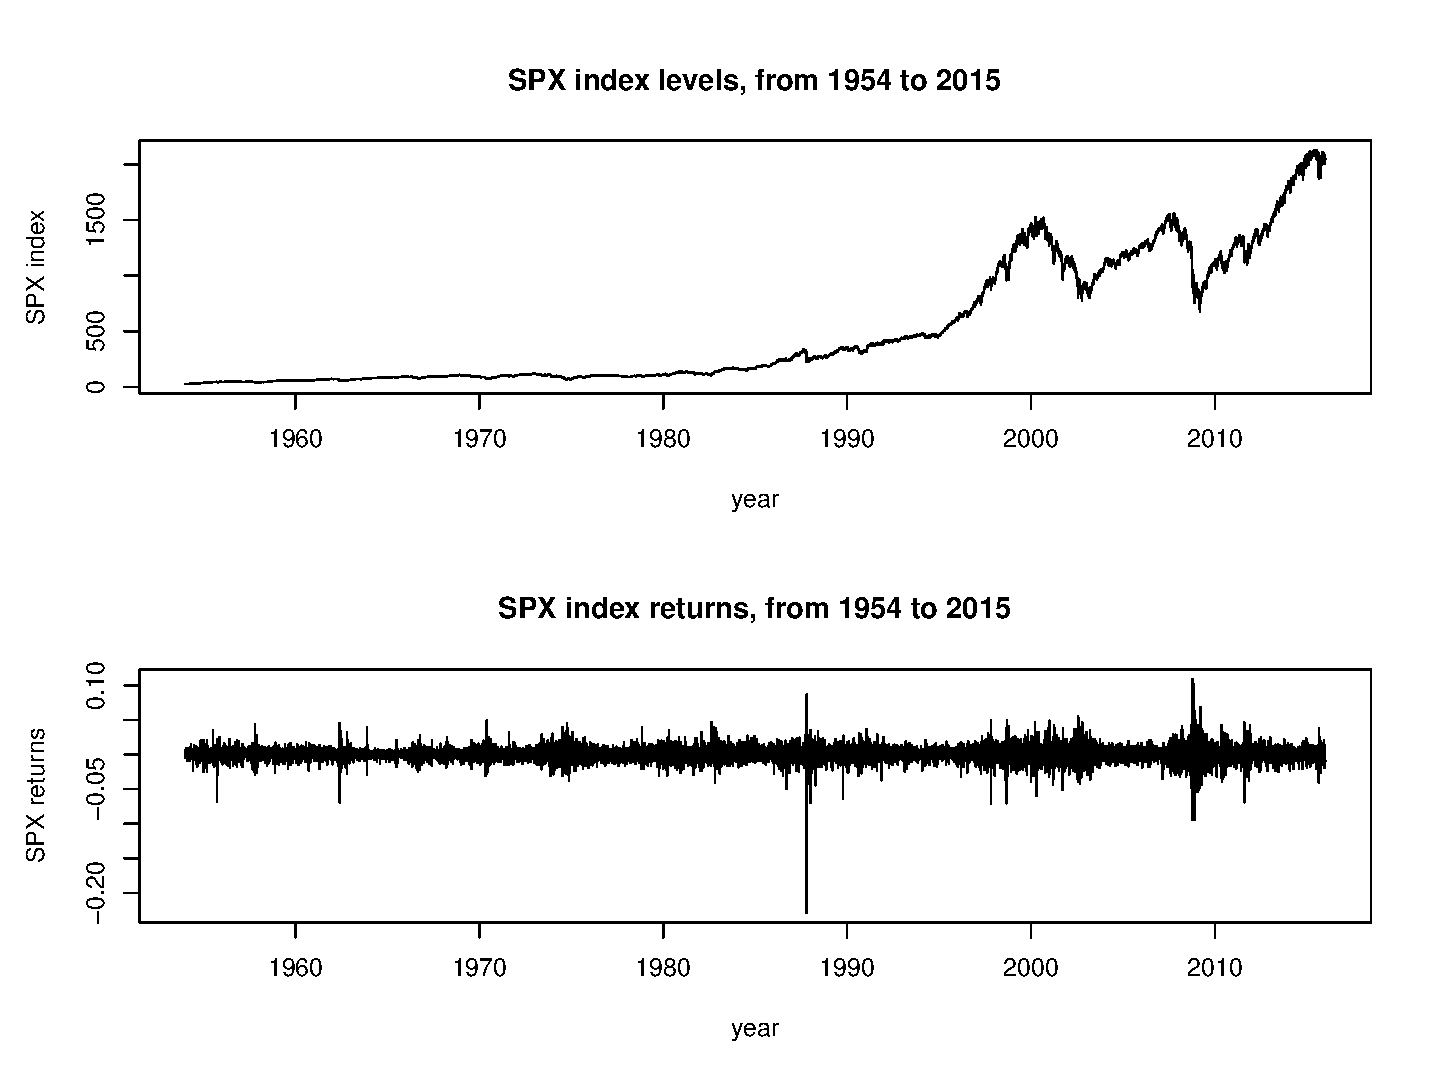
\includegraphics[scale=0.6]{spx_index_return.eps}
  \caption{The SPX index levels and return on daily basis. Time period is from 1954 to 2015.}\label{plot_spx}
\end{figure}

In discrete time equally space, the model has close-form solution for the return
$$
Y_t = \log(S_t / S_{t-1}) = \mu + \sigma \epsilon_t
$$
where $\epsilon_t \sim N(0,1)$. We have $\Theta = (\mu, \sigma^2)$. There is no latent variable, which implies the posterior to be $p(\Theta|Y) = p(\mu,\sigma|Y)$.

Using Hammersley-Clifford theorem~\cite{CH70}, $p(\mu|\sigma^2,Y)$ and $p(\sigma^2|\mu,Y)$ are complete conditionals to the posterior. Assuming independent priors on $\mu$ and $\sigma^2$, Bayes rule implies that
\begin{eqnarray*}
p(\mu|\sigma^2, Y) &\propto& p(Y|\mu,\sigma^2)(\mu) \\
p(\sigma^2|\mu, Y) &\propto& p(Y|\mu,\sigma^2)(\sigma^2) \\
p(Y|\mu,\sigma^2) &=& \left( \frac{1}{\sqrt{2\pi\sigma^2}} \right)^T \exp\left( -\frac{1}{2} \sum_{t=1}^{T} \left( \frac{Y_t - \mu}{\sigma}\right)^2 \right)
\end{eqnarray*}
where $T$ is the sample size. $p(\mu)$ and $p(\sigma^2)$ are priors. Here we choose the standard conjugate priors on $\mu$ and $\sigma^2$. First select the inverse gamma distribution as the prior for $\sigma^2$. The inverse gamma distribution relies on two parameters $\alpha$ and $\beta$. The density is
$$
f(\sigma^2|\alpha,\beta) = \frac{\beta^{\alpha}}{\Gamma(\alpha)} (\sigma^2)^{-\alpha-1} \exp(-\beta/\sigma^2)
$$

Therefore, the marginal density $p(\sigma^2)$ combines the prior $p(\sigma^2)$ and density $p(Y|\mu, \sigma^2)$, which yields

\begin{eqnarray*}
p(\sigma^2|\mu, Y)  &\propto& p(Y|\mu,\sigma^2) \times p(\sigma^2) \\
                    &=& \left( \frac{1}{\sqrt{2\pi\sigma^2}} \right)^T \exp\left( -\frac{1}{2} \sum_{t=1}^{T} \left( \frac{Y_t - \mu}{\sigma}\right)^2 \right) \times \frac{\beta^{\alpha}}{\Gamma(\alpha)} (\sigma^2)^{-\alpha-1} \exp(-\beta/\sigma^2) \\
                    &\propto& (\sigma^2)^{-T/2-\alpha-1} \exp\left( -\left[\frac{1}{2}\sum_{t=1}^{T} (Y_t-\mu)^2 + \beta \right]/\sigma^2 \right) \\
                    &\propto& IG\left(\alpha+\frac{T}{2}, \beta+\frac{1}{2}\sum_{t=1}^{T}(Y_t-\mu)^2 \right)
\end{eqnarray*}

That is, given $\mu$ and $Y_t$, we are able to generate the $\sigma^2$ according to the marginal density $p(\sigma^2|\mu, Y)$. Similarly, select normal distribution as prior for $\mu$. The density is
$$
f(\mu|\theta,\delta) = \frac{1}{\sqrt{2\pi\delta^2}} \exp\left( -frac{1}{2} \left( \frac{\mu-\theta}{\delta} \right)^2 \right)
$$
and the marginal density is
\begin{eqnarray*}
p(\mu|\sigma^2, Y)  &\propto& p(Y|\mu,\sigma^2) \times p(\mu) \\
                    &=& \left( \frac{1}{\sqrt{2\pi\sigma^2}} \right)^T \exp\left( -\frac{1}{2} \sum_{t=1}^{T} \left( \frac{Y_t - \mu}{\sigma}\right)^2 \right) \times \frac{1}{\sqrt{2\pi\delta^2}} \exp\left( -frac{1}{2} \left( \frac{\mu-\theta}{\delta} \right)^2 \right)
\end{eqnarray*}

To deal with $Y_t - \mu$, denote $\hat{\mu}=\left( \sum_{t=1}^T Y_t \right)/T$, and
\begin{eqnarray*}
\sum_{t=1}^T (Y_t - \mu)^2 &=&  \sum_{t=1}^T (Y_t - \hat{\mu} + \hat{\mu} - \mu)^2 \\
                           &=&  \sum_{t=1}^T (Y_t - \hat{\mu})^2 + 2(\hat{\mu}-\mu)\sum_{t=1}^T(Y_t-\hat{\mu}) + \sum_{t=1}^T(\hat{\mu} - \mu)^2 \\
                           &=&  \sum_{t=1}^T (Y_t - \hat{\mu})^2 + T(\hat{\mu}-\mu)^2
\end{eqnarray*}

Continuing on the marginal density, we have
\begin{eqnarray*}
p(\mu|\sigma^2, Y) &\propto& \exp\left(-\frac{T}{2\sigma^2}(\mu-\mu)^2-\frac{1}{2\delta^2}(\mu-\theta)^2\right) \\
                   &\propto& \exp\left(-\frac{T}{2\sigma^2}(-2\hat{\mu}\mu+\mu^2)-\frac{1}{2\delta^2}(\mu^2-2\mu\theta)\right) \\
                   &\propto& \exp\left(-\frac{1}{2\delta^{*2}} \left( \mu-\left(\frac{T\hat{\mu}}{\sigma^2} + \frac{\theta}{\delta^2}\right)\delta^{*2} \right)^2 \right) \\
                   &\propto& N\left( \left( \sum_{t=1}^T Y_t / \sigma^2 + \theta/\delta^2 \right)\delta^{*2}, \delta^{*2} \right)
\end{eqnarray*}
where $\delta^{*2} = (T/\sigma^2+1/\delta^2)^{-1}$.

Given the prior distributions, the complete MCMC method to conduct parameter estimation and statistical inference is
\begin{enumerate}
    \item initialize the parameters $\mu^{(0)}$ and $(\sigma^2)^{0}$;
    \item specify the parameters of the prior $\alpha, \beta, \theta, \delta$;
    \item draw $\mu^{g+1} \sim p(\mu|(\sigma^2)^{g}, Y)$;
    \item draw $(\sigma^2)^{g+1} \sim p(\sigma^2|()^{g}, Y)$;
    \item estimate parameters in $\{\mu^{g}, (\sigma^2)^{g} \}_{g=1}^{G}$ 
\end{enumerate}


\subsection{Merton Jump Diffusion Model}

\section{Data and Empirical Results}

\section{Conclusion}



%
%
%%%%%%%%%%%%%%%%%%%%%%%%%%%%%%%%%%%%%%%%%%%%%%%%%%%
\newpage
\bibliographystyle{plain}
\bibliography{bib}
%%%%%%%%%%%%%%%%%%%%%%%%%%%%%%%%%%%%%%%%%%%%%%%%%%%
%%%%%%%%%%%%%%%%%%%%%%%%%%%%%%%%%%%%%%%%%%%%%%%%%%%
%%%%%%%%%%%%%%%%%%%%%%%%%%%%%%%%%%%%%%%%%%%%%%%%%%%
%
%
%\newpage
%\section*{Appendix: Code for Vasicek model ML estimation}
%%\begin{spacing}{0.9}
%\lstinputlisting[language=R]{assignment1-1.R}

\end{document}
\endinput
